% Abstract for CMSB 2014 poster - BioPreDyn project
\documentclass{llncs}
\usepackage[pdftex, colorlinks=true]{hyperref}
\usepackage{graphicx}
\usepackage{listings}
\usepackage[usenames,dvipsnames]{color}
\begin{document}

\title{BioPreDyn software: an implementation of the systems biology model
building cycle}
\author{Bertrand Moreau \and Eric Boix}
\institute{The CoSMo Company, Lyon, France}
\maketitle

The \href{http://www.biopredyn.eu/}{BioPreDyn} project aims at developing a
software platform integrating several tools specialized in systems biology for
running dry experiments on numerical models. More specifically, this platform
is an implementation of the systems biology model building cycle for data-driven
computational models\cite{Kitano2002}, and allows the execution of simulation
workflows. Current version handles workflows combining simulation run, flux
balance analysis and parameter estimation; its application programming
interface (API) also provides tools for assessing the quality of a numerical
model.

\begin{figure}[!hbtp]
  \centering
  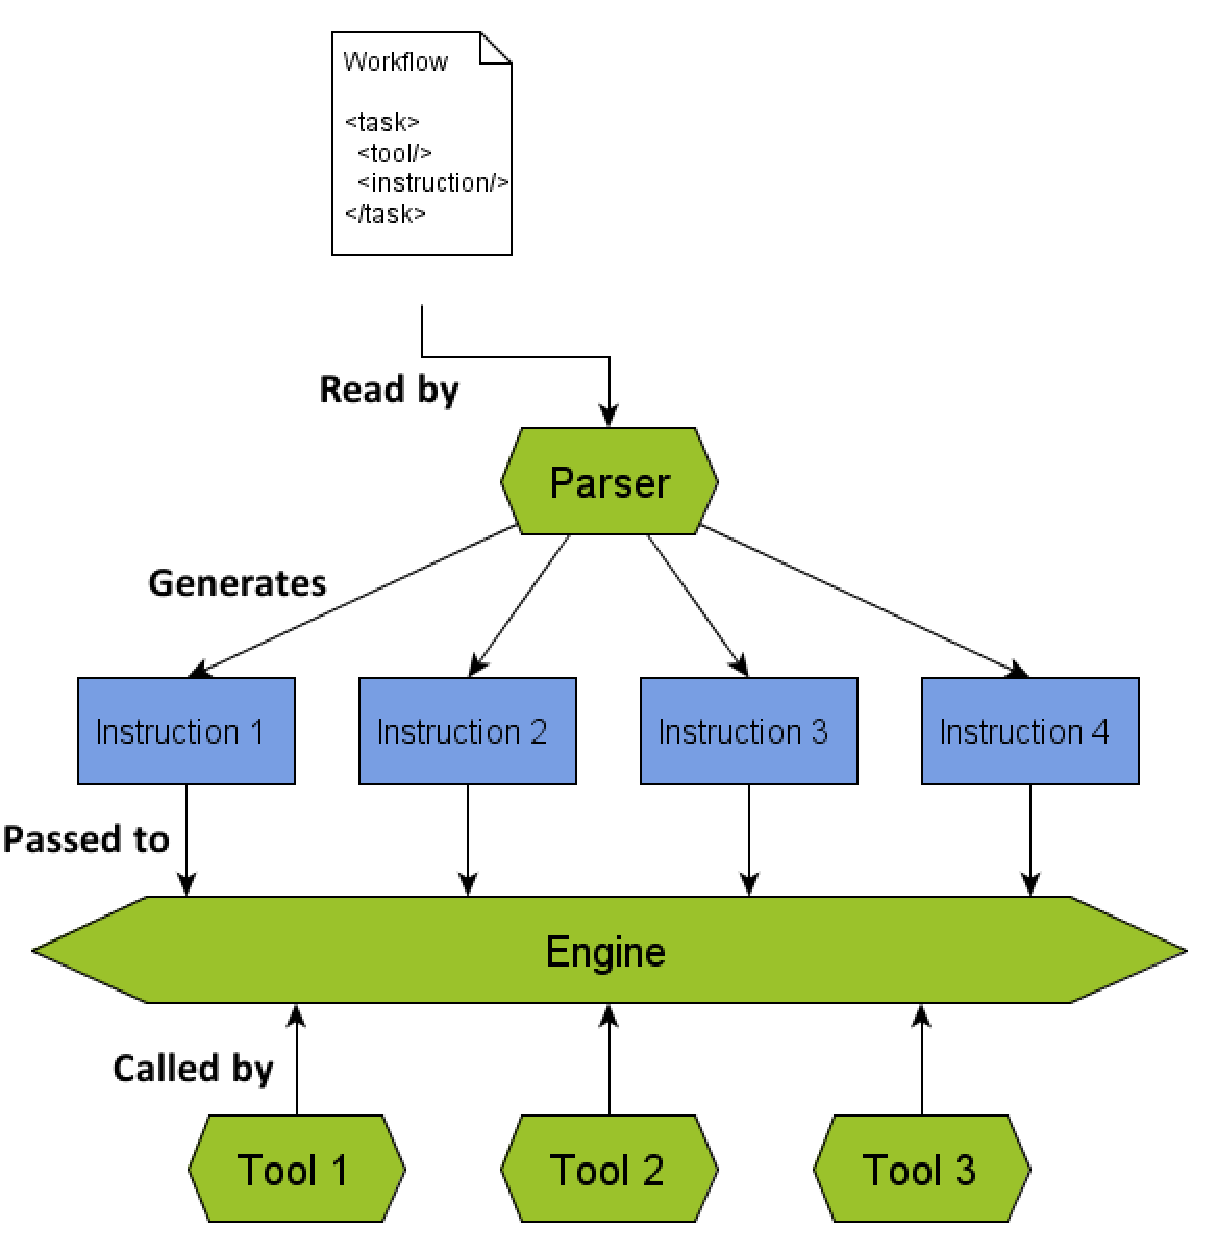
\includegraphics[width=0.5\textwidth]{proposal_complete}
  \caption{Representation of a simulation workflow in BioPreDyn.}
\end{figure}
In the scope of the BioPreDyn project, a simulation workflow - or
numerical experiment - is defined as a sequence of instructions to be executed
on a numerical model; instructions encoded in the workflow include model
initialization, simulation runs and result processing. In this context,
"executing a workflow" simply means executing each instruction sequentially.
Acquiring and parsing the physical representation of the workflow can be part
of the process, as pictured in figure 1. The following standard languages were
chosen to describe the various elements composing a generic model building
workflow:
\begin{enumerate}
\item As a workflow description language: Simulation Experiment Description
Markup Language (\href{http://sed-ml.org/}{SED-ML});
\item As a modeling language: Systems Biology Markup Language
(\href{http://sbml.org}{SBML});
\item As a numerical result description language: Numerical Markup Language
(\href{http://code.google.com/p/numl/}{NuML}), derived from the Systems Biology
Results Markup Language.
\end{enumerate}
With those requirements in mind, an open-source software tool hosted on the
\href{http://www.github.com/bmoreau/biopredyn}{GitHub} platform was developed.
This implementation consists of:
\begin{enumerate}
\item A Python API allowing users to create and edit simulation workflows;
\item Parsers for reading workflows from SED-ML files, describing the tasks,
and passing them to the simulation engine;
\item A Python-based engine capable of dispatching the tasks read by the parsers
to the corresponding simulation tools;
\item A collection of simulation libraries and tools, capable of performing one
or more of the systems biology model building cycle steps.
\end{enumerate}
The BioPreDyn software relies on several tools for writing or reading specific
file formats, running simulations, accessing data bases, etc: dedicated parsers
(libSEDML, libSBML, and libNuML respectively for SED-ML, SBML and NuML files),
simulation engines (libSBMLSim\cite{Takizawa2013}, CobraPY\cite{Ebrahim2013}
and COPASI\cite{Hoops2006}), web services (BioServices\cite{Cokelaer2013}).
Depending on the task to be done, the user can therefore choose between
different simulation engines.\\

The BioPreDyn software can be used as any Python library for scripting more
elaborated workflows:
\lstinputlisting[
  language=Python,
  basicstyle=\footnotesize\ttfamily,
  keywordstyle=\color{ForestGreen},
  commentstyle=\color{Gray},
  stringstyle=\color{Fuchsia}]{script_example.py}
\bibliography{references}{}
\bibliographystyle{splncs03}
\end{document}
